
%% bare_jrnl.tex
%% V1.4b
%% 2015/08/26
%% by Michael Shell
%% see http://www.michaelshell.org/
%% for current contact information.
%%
%% This is a skeleton file demonstrating the use of IEEEtran.cls
%% (requires IEEEtran.cls version 1.8b or later) with an IEEE
%% journal paper.
%%
%% Support sites:
%% http://www.michaelshell.org/tex/ieeetran/
%% http://www.ctan.org/pkg/ieeetran
%% and
%% http://www.ieee.org/

%%*************************************************************************
%% Legal Notice:
%% This code is offered as-is without any warranty either expressed or
%% implied; without even the implied warranty of MERCHANTABILITY or
%% FITNESS FOR A PARTICULAR PURPOSE! 
%% User assumes all risk.
%% In no event shall the IEEE or any contributor to this code be liable for
%% any damages or losses, including, but not limited to, incidental,
%% consequential, or any other damages, resulting from the use or misuse
%% of any information contained here.
%%
%% All comments are the opinions of their respective authors and are not
%% necessarily endorsed by the IEEE.
%%
%% This work is distributed under the LaTeX Project Public License (LPPL)
%% ( http://www.latex-project.org/ ) version 1.3, and may be freely used,
%% distributed and modified. A copy of the LPPL, version 1.3, is included
%% in the base LaTeX documentation of all distributions of LaTeX released
%% 2003/12/01 or later.
%% Retain all contribution notices and credits.
%% ** Modified files should be clearly indicated as such, including  **
%% ** renaming them and changing author support contact information. **
%%*************************************************************************


% *** Authors should verify (and, if needed, correct) their LaTeX system  ***
% *** with the testflow diagnostic prior to trusting their LaTeX platform ***
% *** with production work. The IEEE's font choices and paper sizes can   ***
% *** trigger bugs that do not appear when using other class files.       ***                          ***
% The testflow support page is at:
% http://www.michaelshell.org/tex/testflow/



\documentclass[journal]{IEEEtran}
%
% If IEEEtran.cls has not been installed into the LaTeX system files,
% manually specify the path to it like:
% \documentclass[journal]{../sty/IEEEtran}



% Some very useful LaTeX packages include:
% (uncomment the ones you want to load)


% *** GRAPHICS RELATED PACKAGES ***
%
\ifCLASSINFOpdf
  % \usepackage[pdftex]{graphicx}
  % declare the path(s) where your graphic files are
  % \graphicspath{{../pdf/}{../jpeg/}}
  % and their extensions so you won't have to specify these with
  % every instance of \includegraphics
  % \DeclareGraphicsExtensions{.pdf,.jpeg,.png}
\else
  % or other class option (dvipsone, dvipdf, if not using dvips). graphicx
  % will default to the driver specified in the system graphics.cfg if no
  % driver is specified.
  % \usepackage[dvips]{graphicx}
  % declare the path(s) where your graphic files are
  % \graphicspath{{../eps/}}
  % and their extensions so you won't have to specify these with
  % every instance of \includegraphics
  % \DeclareGraphicsExtensions{.eps}
\fi
% graphicx was written by David Carlisle and Sebastian Rahtz. It is
% required if you want graphics, photos, etc. graphicx.sty is already
% installed on most LaTeX systems. The latest version and documentation
% can be obtained at: 
% http://www.ctan.org/pkg/graphicx
% Another good source of documentation is "Using Imported Graphics in
% LaTeX2e" by Keith Reckdahl which can be found at:
% http://www.ctan.org/pkg/epslatex
%
% latex, and pdflatex in dvi mode, support graphics in encapsulated
% postscript (.eps) format. pdflatex in pdf mode supports graphics
% in .pdf, .jpeg, .png and .mps (metapost) formats. Users should ensure
% that all non-photo figures use a vector format (.eps, .pdf, .mps) and
% not a bitmapped formats (.jpeg, .png). The IEEE frowns on bitmapped formats
% which can result in "jaggedy"/blurry rendering of lines and letters as
% well as large increases in file sizes.
%
% You can find documentation about the pdfTeX application at:
% http://www.tug.org/applications/pdftex





% *** MATH PACKAGES ***
%
%\usepackage{amsmath}
% A popular package from the American Mathematical Society that provides
% many useful and powerful commands for dealing with mathematics.
%
% Note that the amsmath package sets \interdisplaylinepenalty to 10000
% thus preventing page breaks from occurring within multiline equations. Use:
%\interdisplaylinepenalty=2500
% after loading amsmath to restore such page breaks as IEEEtran.cls normally
% does. amsmath.sty is already installed on most LaTeX systems. The latest
% version and documentation can be obtained at:
% http://www.ctan.org/pkg/amsmath






% IEEEtran contains the IEEEeqnarray family of commands that can be used to
% generate multiline equations as well as matrices, tables, etc., of high
% quality.



% *** FLOAT PACKAGES ***
%
%\usepackage{fixltx2e}
% fixltx2e, the successor to the earlier fix2col.sty, was written by
% Frank Mittelbach and David Carlisle. This package corrects a few problems
% in the LaTeX2e kernel, the most notable of which is that in current
% LaTeX2e releases, the ordering of single and double column floats is not
% guaranteed to be preserved. Thus, an unpatched LaTeX2e can allow a
% single column figure to be placed prior to an earlier double column
% figure.
% Be aware that LaTeX2e kernels dated 2015 and later have fixltx2e.sty's
% corrections already built into the system in which case a warning will
% be issued if an attempt is made to load fixltx2e.sty as it is no longer
% needed.
% The latest version and documentation can be found at:
% http://www.ctan.org/pkg/fixltx2e


%\usepackage{stfloats}
% stfloats.sty was written by Sigitas Tolusis. This package gives LaTeX2e
% the ability to do double column floats at the bottom of the page as well
% as the top. (e.g., "\begin{figure*}[!b]" is not normally possible in
% LaTeX2e). It also provides a command:
%\fnbelowfloat
% to enable the placement of footnotes below bottom floats (the standard
% LaTeX2e kernel puts them above bottom floats). This is an invasive package
% which rewrites many portions of the LaTeX2e float routines. It may not work
% with other packages that modify the LaTeX2e float routines. The latest
% version and documentation can be obtained at:
% http://www.ctan.org/pkg/stfloats
% Do not use the stfloats baselinefloat ability as the IEEE does not allow
% \baselineskip to stretch. Authors submitting work to the IEEE should note
% that the IEEE rarely uses double column equations and that authors should try
% to avoid such use. Do not be tempted to use the cuted.sty or midfloat.sty
% packages (also by Sigitas Tolusis) as the IEEE does not format its papers in
% such ways.
% Do not attempt to use stfloats with fixltx2e as they are incompatible.
% Instead, use Morten Hogholm'a dblfloatfix which combines the features
% of both fixltx2e and stfloats:
%
% \usepackage{dblfloatfix}
% The latest version can be found at:
% http://www.ctan.org/pkg/dblfloatfix




%\ifCLASSOPTIONcaptionsoff
%  \usepackage[nomarkers]{endfloat}
% \let\MYoriglatexcaption\caption
% \renewcommand{\caption}[2][\relax]{\MYoriglatexcaption[#2]{#2}}
%\fi
% endfloat.sty was written by James Darrell McCauley, Jeff Goldberg and 
% Axel Sommerfeldt. This package may be useful when used in conjunction with 
% IEEEtran.cls'  captionsoff option. Some IEEE journals/societies require that
% submissions have lists of figures/tables at the end of the paper and that
% figures/tables without any captions are placed on a page by themselves at
% the end of the document. If needed, the draftcls IEEEtran class option or
% \CLASSINPUTbaselinestretch interface can be used to increase the line
% spacing as well. Be sure and use the nomarkers option of endfloat to
% prevent endfloat from "marking" where the figures would have been placed
% in the text. The two hack lines of code above are a slight modification of
% that suggested by in the endfloat docs (section 8.4.1) to ensure that
% the full captions always appear in the list of figures/tables - even if
% the user used the short optional argument of \caption[]{}.
% IEEE papers do not typically make use of \caption[]'s optional argument,
% so this should not be an issue. A similar trick can be used to disable
% captions of packages such as subfig.sty that lack options to turn off
% the subcaptions:
% For subfig.sty:
% \let\MYorigsubfloat\subfloat
% \renewcommand{\subfloat}[2][\relax]{\MYorigsubfloat[]{#2}}
% However, the above trick will not work if both optional arguments of
% the \subfloat command are used. Furthermore, there needs to be a
% description of each subfigure *somewhere* and endfloat does not add
% subfigure captions to its list of figures. Thus, the best approach is to
% avoid the use of subfigure captions (many IEEE journals avoid them anyway)
% and instead reference/explain all the subfigures within the main caption.
% The latest version of endfloat.sty and its documentation can obtained at:
% http://www.ctan.org/pkg/endfloat
%
% The IEEEtran \ifCLASSOPTIONcaptionsoff conditional can also be used
% later in the document, say, to conditionally put the References on a 
% page by themselves.


% correct bad hyphenation here
\hyphenation{cons-trição constri-ção}

\usepackage[utf8]{inputenc} %codificação do texto
\usepackage[T1]{fontenc} %queremos acentuação, né?!
\usepackage{hyperref} %para adicionar hiperlink
\usepackage{graphicx}

\begin{document}
%
% paper title
\title{Maximização de Doentes em um quarto minimizando o contágio usando PSO}
%
%
% author names and IEEE memberships
% note positions of commas and nonbreaking spaces ( ~ ) LaTeX will not break
% a structure at a ~ so this keeps an author's name from being broken across
% two lines.
% use \thanks{} to gain access to the first footnote area
% a separate \thanks must be used for each paragraph as LaTeX2e's \thanks
% was not built to handle multiple paragraphs
%

\author{Barros, G. P. - Escola Politécnica de Pernambuco. UPE
	Recife - PE.\\
	gpb@ecomp.poli.br\\
	\and
	Silva, I.A. - Escola Politécnica de Pernambuco. UPE
	Recife - PE.\\
	ias@ecomp.poli.br%
}%

% note the % following the last \IEEEmembership and also \thanks - 
% these prevent an unwanted space from occurring between the last author name
% and the end of the author line. i.e., if you had this:
% 
% \author{....lastname \thanks{...} \thanks{...} }
%                     ^------------^------------^----Do not want these spaces!
%

% The paper headers
\markboth{Inteligência de Enxames - Projeto - Prof Carmelo Bastos}%
{Inteligência de Enxames - Projeto}
% The only time the second header will appear is for the odd numbered pages
% after the title page when using the twoside option. 

% make the title area
\maketitle

% As a general rule, do not put math, special symbols or citations
% in the abstract or keywords.
\begin{abstract}
Para prevenir e controlar a disseminação de doenças infecto-contagiosas em ambiente hospitalar adotam-se precauções de acordo com os tipos das mesmas. Neste projeto, objetivou-se determinar, mediante o uso da técnica \textit{Particle Swarm Optimization}	(PSO), o maior arranjo possível de pacientes com doenças infecto-contagiosas em um quarto, de tal forma que a possibilidade do contágio seja o mínimizada. 
\end{abstract}

% Note that keywords are not normally used for peerreview papers.
\begin{IEEEkeywords}
PSO, swarm optimization, disease.
\end{IEEEkeywords}



% For peer review papers, you can put extra information on the cover
% page as needed:
% \ifCLASSOPTIONpeerreview
% \begin{center} \bfseries EDICS Category: 3-BBND \end{center}
% \fi
%
% For peerreview papers, this IEEEtran command inserts a page break and
% creates the second title. It will be ignored for other modes.
\IEEEpeerreviewmaketitle



\section{Introdução}
% The very first letter is a 2 line initial drop letter followed
% by the rest of the first word in caps.
% 
% form to use if the first word consists of a single letter:
% \IEEEPARstart{A}{demo} file is ....
% 
% form to use if you need the single drop letter followed by
% normal text (unknown if ever used by the IEEE):
% \IEEEPARstart{A}{}demo file is ....
% 
% Some journals put the first two words in caps:
% \IEEEPARstart{T}{his demo} file is ....
% 
% Here we have the typical use of a "T" for an initial drop letter
% and "HIS" in caps to complete the first word.
% You must have at least 2 lines in the paragraph with the drop letter
% (should never be an issue)
\IEEEPARstart{N}{a} ultima década o mundo testemunhou um surto global de doenças infecto-contagiosas. Entre diversos fatores, o aumento de atividades econômicas nas cidades pode atrair pessoas das áreas rurais para as grandes cidades, assim como pode atrair pessoas de outros países, onde, este grande movimento pode gerar grandes riscos em relação a transmissão de doenças \cite{Inayatulloh:2015} e ocasionar o aumento de pacientes nos hospitais. É fato que o ambiente hospitalar é propício ao risco aumentado da aquisição e transmissão de infecção por disseminação de microorganismos, como bactérias resistentes e outros agentes causadores de doenças infecto-contagiosas \cite{Ribeiro:2008}. No entanto, o problema está na transmissão dessas bactérias e microorganismos para pacientes sucetíveis (estão com baixa imunidade) e para os profissionais de saúde que também convivem neste ambiente \footnote[1]{\emph{Isolamento e Precauções} \url{http://www.ufmt.br/hujm/arquivos/7e18458a8aa832719641156ccd469de8.pdf}. Último acesso em 8 de junho de 2016.}\par%
As emergências médicas abrigam tanto adultos (mulheres e homens) quanto crianças, sem distinção, onde, o risco do contágio mostra a importância de utilizar métodos inteligentes em busca de diminuir este problema ao máximo. Em busca de minimizar o contágio entre os pacientes em ambiente médico é proposto, neste projeto, a utilização do algoritmo \textit{Particle Swarm Optimization} (PSO) com o objetivo de determinar arranjos com a maior quantidade de pacientes em um quarto.\par%
O PSO foi introduzido por \cite{Kennedy:1995} e surgiu de experiências com algoritmos modelados a partir da observação do comportamento social de determinadas espécies de pássaros \cite{Siciliano:2007}. As partículas consideradas pelo algoritmo se comportam como os pássaros à procura de alimento ou do local de seus ninhos, utilizando o aprendizado próprio e o aprendizado do enxame. O PSO é composto de partículas representadas por vetores que constituem a velocidade e posição atual de cada partícula, que são atualizados segundo a velocidade atual, seu aprendizado pessoal e o aprendizado adquirido pelo bando que são descritos como termos cognitivos e sociais, respectivamente \cite{Siciliano:2007}.\par%
  

% needed in second column of first page if using \IEEEpubid
%\IEEEpubidadjcol

% An example of a floating figure using the graphicx package.
% Note that \label must occur AFTER (or within) \caption.
% For figures, \caption should occur after the \includegraphics.
% Note that IEEEtran v1.7 and later has special internal code that
% is designed to preserve the operation of \label within \caption
% even when the captionsoff option is in effect. However, because
% of issues like this, it may be the safest practice to put all your
% \label just after \caption rather than within \caption{}.
%
% Reminder: the "draftcls" or "draftclsnofoot", not "draft", class
% option should be used if it is desired that the figures are to be
% displayed while in draft mode.
%
%\begin{figure}[!t]
%\centering
%\includegraphics[width=2.5in]{myfigure}
% where an .eps filename suffix will be assumed under latex, 
% and a .pdf suffix will be assumed for pdflatex; or what has been declared
% via \DeclareGraphicsExtensions.
%\caption{Simulation results for the network.}
%\label{fig_sim}
%\end{figure}

% Note that the IEEE typically puts floats only at the top, even when this
% results in a large percentage of a column being occupied by floats.


% An example of a double column floating figure using two subfigures.
% (The subfig.sty package must be loaded for this to work.)
% The subfigure \label commands are set within each subfloat command,
% and the \label for the overall figure must come after \caption.
% \hfil is used as a separator to get equal spacing.
% Watch out that the combined width of all the subfigures on a 
% line do not exceed the text width or a line break will occur.
%
%\begin{figure*}[!t]
%\centering
%\subfloat[Case I]{\includegraphics[width=2.5in]{box}%
%\label{fig_first_case}}
%\hfil
%\subfloat[Case II]{\includegraphics[width=2.5in]{box}%
%\label{fig_second_case}}
%\caption{Simulation results for the network.}
%\label{fig_sim}
%\end{figure*}
%
% Note that often IEEE papers with subfigures do not employ subfigure
% captions (using the optional argument to \subfloat[]), but instead will
% reference/describe all of them (a), (b), etc., within the main caption.
% Be aware that for subfig.sty to generate the (a), (b), etc., subfigure
% labels, the optional argument to \subfloat must be present. If a
% subcaption is not desired, just leave its contents blank,
% e.g., \subfloat[].


% An example of a floating table. Note that, for IEEE style tables, the
% \caption command should come BEFORE the table and, given that table
% captions serve much like titles, are usually capitalized except for words
% such as a, an, and, as, at, but, by, for, in, nor, of, on, or, the, to
% and up, which are usually not capitalized unless they are the first or
% last word of the caption. Table text will default to \footnotesize as
% the IEEE normally uses this smaller font for tables.
% The \label must come after \caption as always.
%
%\begin{table}[!t]
%% increase table row spacing, adjust to taste
%\renewcommand{\arraystretch}{1.3}
% if using array.sty, it might be a good idea to tweak the value of
% \extrarowheight as needed to properly center the text within the cells
%\caption{An Example of a Table}
%\label{table_example}
%\centering
%% Some packages, such as MDW tools, offer better commands for making tables
%% than the plain LaTeX2e tabular which is used here.
%\begin{tabular}{|c||c|}
%\hline
%One & Two\\
%\hline
%Three & Four\\
%\hline
%\end{tabular}
%\end{table}


\section{Título de uma seção}
\subsection{Sistema Operacional}
Ubuntu 16.04 LTS. 64-bit.\textit{ Testes e relatório }\par
Windows 7. 64-bit.\textit{ Desenvolvimento}
\subsection{Processador}
Intel Core i5-2430M CPU @ 2.40GHz x 4\par
Intel Core i7-K875 CPU @ 2.93GHz x 8
\subsection{Linguagem}
Projeto feito em Java, usando o Netbeans como IDE, sem o uso de bibliotecas externas que façam o que é proposto na atividade.\\A versão digital deste documento, pode ser encontrado em \url{https://github.com/iagows/Enxames_Entrega_4/tree/master/artigo}.%

\section{Função}
Descrever a função.
\subsection{Distância}
$f(x)=\sum\limits_{i=1}^{D}|\sqrt[2]{(x_i - x_k)^2 - (y_i - y_k)^2} - (R_i - R_k)|$

\section{Algoritmos}
Os algoritmos em teste são: PSO usando o fator de constrição de Clerc, ABC e FSS.

\section{Experimentos}
Os dados dos experimentos são como vistos na tabela \ref{table:prop}.\par
No ABC e no FSS, as partículas são as abelhas e os peixes, respectivamente.
\begin{table}
\renewcommand{\arraystretch}{1.3}
\caption{Propriedades}
\label{table:prop}
\centering
\begin{tabular}{c|c}
    \hline
    Nome  &  Valor\\
    \hline
    \hline

    Partículas & 30\\
    \hline
    Dimensões & 30\\
    \hline
    Iterações & 10.000\\
    \hline
\end{tabular}
\end{table}

\section{Resultados esperados}
Texto.%

\section{Resultados}
Texto.%

\subsection{Esfera}
\begin{figure}
	\centering
	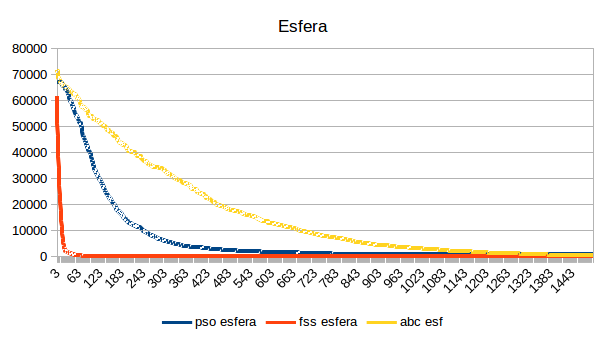
\includegraphics[width=0.4\textwidth]{img/esf}
	\caption{Benchmark na função esfera}
	\label{fig:esfera}
\end{figure}
\begin{figure}
	\centering
	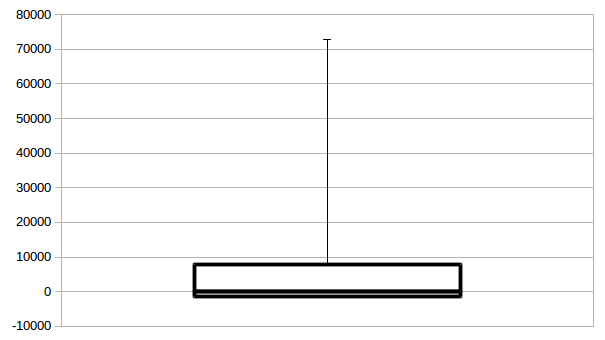
\includegraphics[width=0.4\textwidth]{img/block_esf}
	\caption{Boxplot da função Esfera}
	\label{fig:besf}
\end{figure}
Figura \ref{fig:esfera}. Figura \ref{fig:besf}.


\section{Conclusão}
Bla.%

\section{Trabalhos Futuros}
Bla.%

% Can use something like this to put references on a page
% by themselves when using endfloat and the captionsoff option.
%\ifCLASSOPTIONcaptionsoff
%  \newpage
%\fi



% trigger a \newpage just before the given reference
% number - used to balance the columns on the last page
% adjust value as needed - may need to be readjusted if
% the document is modified later
%\IEEEtriggeratref{8}
% The "triggered" command can be changed if desired:
%\IEEEtriggercmd{\enlargethispage{-5in}}

% references section

\begin{thebibliography}{1}

\bibitem{CARMELO:2008}
Carmelo J.A. Bastos-Filho, Fernando B. Lima-Neto, Anthony J.C.C. Lins, Antônio I.S. Nascimento, Marília P. Lima.\emph{A novel search algorithm based on fish school behavior}, Conference Paper.\hskip 1em plus 0.5em minus 0.4em\relax Departamento de Sistemas Computacionais, Escola Politécnica de Pernambuco. Recife-PE, Brasil, 2008.%

\bibitem{Karaboga:2005}
D. Dervis Karaboga. \emph{An Idea Based On Honey Bee Swarm for Numerical Optimization}, Technical Report. \hskip 1em plus 0.5em minus 0.4em\relax -TR06,Erciyes University, Engineering Faculty, Computer Engineering Department 2005.%

\bibitem{Inayatulloh:2015}
Inayatulloh; Theresia, S. \emph{Early Warning System for Infectious Diseases}, \hskip 1em plus 0.5em minus 0.4em\relax -TR06,Bina Nusantara University, School of Information Systems. Indonesia. 2015.%

\bibitem{Iago:2016}
Silva, I.A. \emph{Análise de Desempenho de PSO: Benchmark Tool} \hskip 1em plus 0.5em minus 0.4em\relax Prática número 1, Inteligência de Enxames. \url{https://github.com/iagows/simple_pso/blob/master/artigo/Artigo.pdf} Último acesso em 1 de maio de 2016.%

\bibitem{Kennedy:1995}
Kennedy, J.; Eberhart, R.\emph{Particle Swarm Optimization}. \relax Proceedings of IEEE International Conference on Neural Networks. pp. 1942–1948. 1995.%

\bibitem{Ribeiro:2008}
Ribeiro, M. R.; Rezende, E. M.; Neves, F. C.; Clemente, W. T.; Souza, P. C.; Brandão, G. S. \relax Indicação de Precauções de Acordo com as Vias de Transmissão para Portadores de Bactéria Resistente. 2008.%

\bibitem{Siciliano:2007}
Siciliano, A. V. \relax Algoritmos Genéticos e Particle Swarm Optimization e suas aplicações em problemas de Guerra Eletrônica.In: IX Simpósio de Guerra Eletrônica, 2007, São José dos Campos (ITA).% 

  
%\bibitem{Artigo:fulano}
%Completo, Nome do Fulano, \emph{Nome do artigo}, edição.\hskip 1em plus 0.5em minus 0.4em \relax Cidade, País: universidade, ano.

\end{thebibliography}


%\begin{IEEEbiographynophoto}{Iago Alves}
%Formado em Engenharia da Computação pela Escola Politécnica de Pernambuco. Atualmente é aluno %ouvinte no mestrado do curso supracitado.
%\end{IEEEbiographynophoto}



% that's all folks
\end{document}